%!TEX TS-program = xelatex
%!TEX encoding = UTF-8 Unicode

% Author: Romain "Artefact2" Dal Maso <artefact2@gmail.com>
% 
% This program is free software. It comes without any warranty, to the
% extent permitted by applicable law. You can redistribute it and/or
% modify it under the terms of the Do What The Fuck You Want To Public
% License, Version 2, as published by Sam Hocevar. See
% http://sam.zoy.org/wtfpl/COPYING for more details.

\newcolumntype{L}{>{\small\scaly}l}
\newcolumntype{C}{>{\small\scaly}c}
\newcolumntype{R}{>{\small\scaly}r}
\newcolumntype{Y}{>{\small\scaly}X}
\newcolumntype{Z}{>{\small\scaly\centering\arraybackslash}X}

\newlength{\hbTableBorderX}
\newlength{\hbTableBorderY}
\newlength{\hbTableBorderS}
\newlength{\hbTableBoxWidth}
\newlength{\hbTableBoxHeight}
\newlength{\hbTableBoxDepth}
\newsavebox{\hbTableBox}

\setlength{\hbTableBorderX}{10pt}
\setlength{\hbTableBorderY}{14pt}
\setlength{\hbTableBorderS}{5em}

\renewcommand*{\arraystretch}{1.1}

\captionstyle{\raggedright}
\captiondelim{}
\captionnamefont{\fontsize{1sp}{0pt}\selectfont} % XXX: hackish
\captiontitlefont{\scaly\scshape\bfseries\large}

\newcommand*{\hbTableBefore}{%
  \global\rownum=0%
  \rowcolors{1}{}{note}%
}

\newcommand*{\hbTableDrawFancy}{%
    \settowidth{\hbTableBoxWidth}{\usebox{\hbTableBox}}%
    \settoheight{\hbTableBoxHeight}{\usebox{\hbTableBox}}%
    \settodepth{\hbTableBoxDepth}{\usebox{\hbTableBox}}%
    \TPoptions{absolute=false}%
    \noindent\vspace*{\hbTableBorderY}%
    \begin{textblock*}{\linewidth}(-\hbTableBorderX,-\hbTableBorderY)%
    \scalebox{-1}[1]{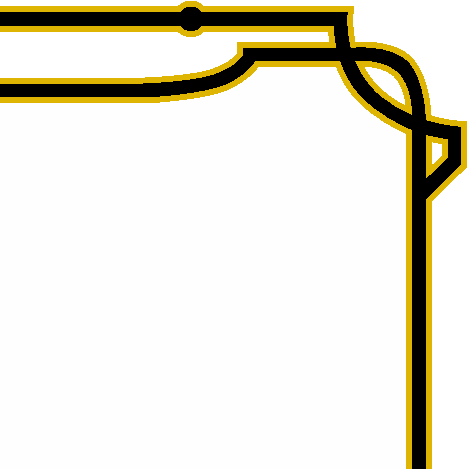
\includegraphics[width=\hbTableBorderS,height=\hbTableBorderS]{assets/fancy-table-corner}}
    \end{textblock*}%
    \begin{textblock*}{\linewidth}(\hbTableBoxWidth-\hbTableBorderS+\hbTableBorderX,-\hbTableBorderY)%
    \scalebox{1}[1]{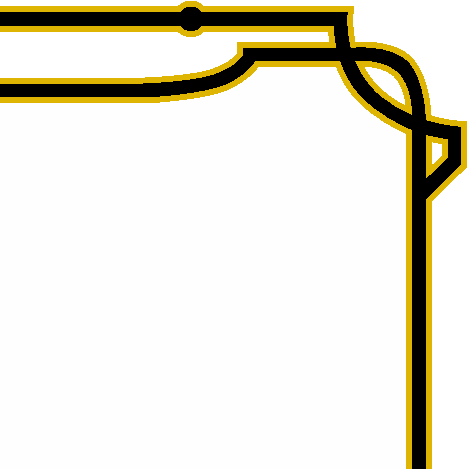
\includegraphics[width=\hbTableBorderS,height=\hbTableBorderS]{assets/fancy-table-corner}}
    \end{textblock*}%
    \begin{textblock*}{\linewidth}(-\hbTableBorderX,\hbTableBoxHeight+\hbTableBoxDepth-\hbTableBorderS+\hbTableBorderY)%
    \scalebox{-1}[-1]{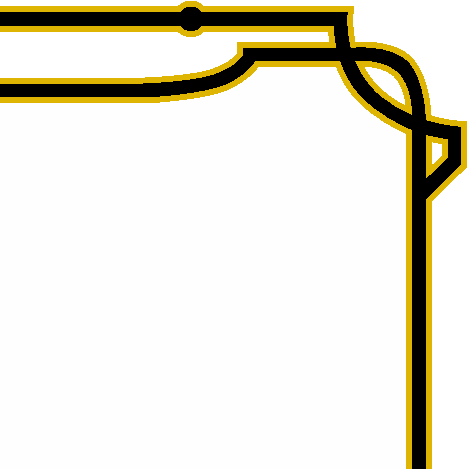
\includegraphics[width=\hbTableBorderS,height=\hbTableBorderS]{assets/fancy-table-corner}}
    \end{textblock*}%
    \begin{textblock*}{\linewidth}(\hbTableBoxWidth-\hbTableBorderS+\hbTableBorderX,\hbTableBoxHeight+\hbTableBoxDepth-\hbTableBorderS+\hbTableBorderY)%
    \scalebox{1}[-1]{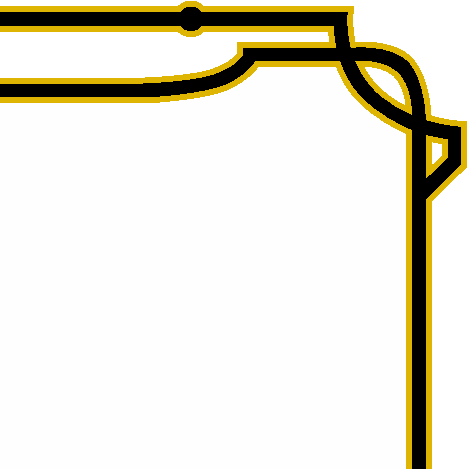
\includegraphics[width=\hbTableBorderS,height=\hbTableBorderS]{assets/fancy-table-corner}}
    \end{textblock*}%
    \begin{textblock*}{\linewidth}(-\hbTableBorderX+\hbTableBorderS,-\hbTableBorderY)%
    \scalebox{1}[1]{
\includegraphics[height=\hbTableBorderS,width=\hbTableBoxWidth-2\hbTableBorderS+2\hbTableBorderX]{assets/fancy-table-vert}}
    \end{textblock*}%
    \begin{textblock*}{\linewidth}(-\hbTableBorderX+\hbTableBorderS,\hbTableBoxHeight+\hbTableBoxDepth-\hbTableBorderS+\hbTableBorderY)%
    \scalebox{1}[-1]{
\includegraphics[height=\hbTableBorderS,width=\hbTableBoxWidth-2\hbTableBorderS+2\hbTableBorderX]{assets/fancy-table-vert}}
    \end{textblock*}%
    \begin{textblock*}{\linewidth}(-\hbTableBorderX,-\hbTableBorderY+\hbTableBorderS)%
    \scalebox{-1}[1]{
\includegraphics[height=\hbTableBoxHeight+\hbTableBoxDepth-2\hbTableBorderS+2\hbTableBorderY,width=\hbTableBorderS]{assets/fancy-table-horiz}}
    \end{textblock*}%
    \begin{textblock*}{\linewidth}(\hbTableBoxWidth-\hbTableBorderS+\hbTableBorderX,-\hbTableBorderY+\hbTableBorderS)%
    \scalebox{1}[1]{
\includegraphics[height=\hbTableBoxHeight+\hbTableBoxDepth-2\hbTableBorderS+2\hbTableBorderY,width=\hbTableBorderS]{assets/fancy-table-horiz}}
    \end{textblock*}%
    \usebox{\hbTableBox}\vspace*{\hbTableBorderY}%
    \TPoptions{absolute=true}%
}

\NewEnviron{hbNakedTable}[1]{%
  \hbTableBefore%
  \medbreak\noindent\begin{tabularx}{\linewidth}{#1}\BODY\end{tabularx}\medbreak%
}

\NewEnviron{hbNarrowTable}[3][h]{%
  \begin{table}[#1]%
    \caption{#2}%
    \hbTableBefore%
    \noindent\begin{tabularx}{\linewidth}{#3}\BODY\end{tabularx}%
  \end{table}%
}

\NewEnviron{hbWideTable}[3][t]{%
  \begin{table*}[#1]%
    \caption{#2}%
    \hbTableBefore%
    \noindent\begin{tabularx}{\linewidth}{#3}\BODY\end{tabularx}%
  \end{table*}%
}

\NewEnviron{hbFancyTable}[3][h]{%
  \begin{table}[#1]%
    \hbTableBefore%
    \sbox{\hbTableBox}{\colorbox{white}{\begin{minipage}{\linewidth-2\fboxsep}%
    \caption{#2}%
    \begin{tabularx}{\linewidth}{#3}\BODY\end{tabularx}%
    \end{minipage}}}%
    \hbTableDrawFancy%
  \end{table}%
}

\NewEnviron{hbFancyWideTable}[3][t]{%
  \begin{table*}[#1]%
    \hbTableBefore%
    \sbox{\hbTableBox}{\colorbox{white}{\begin{minipage}{\linewidth-2\fboxsep}%
    \caption{#2}%
    \begin{tabularx}{\linewidth}{#3}\BODY\end{tabularx}%
    \end{minipage}}}%
    \hbTableDrawFancy%
  \end{table*}%
}
